\chapter{Annexes}

\section*{Timer.cs}
\lstinputlisting{../../unity/project/Assets/Engine/Timer.cs}
\section*{BeatCounter.cs}
\lstinputlisting{../../unity/project/Assets/Engine/BeatCounter.cs}

\section*{Extrait de la table de code midi}
\begin{figure}[H]\centering
  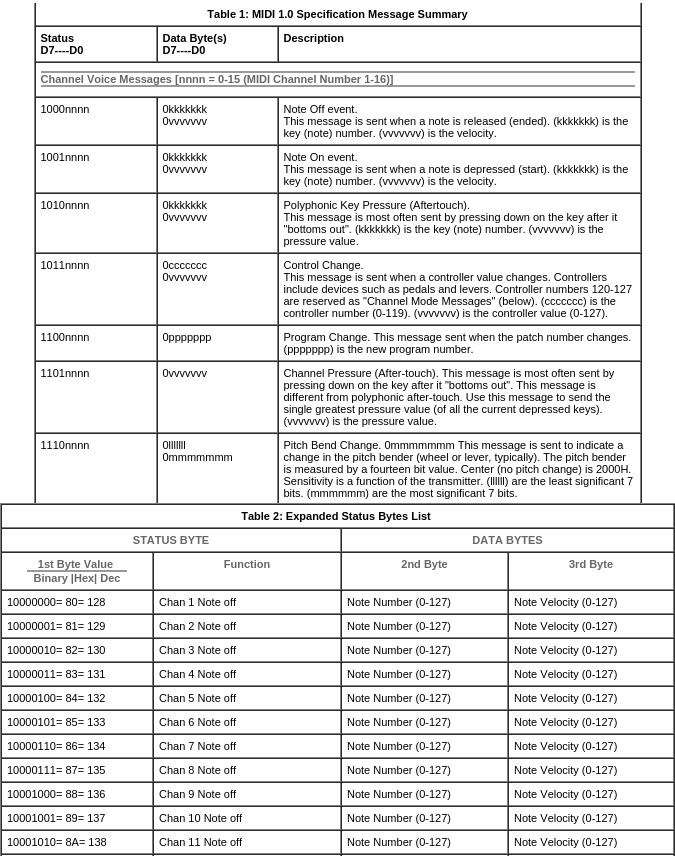
\includegraphics[scale=0.8]{./img/midi_spec.png}
  \caption{Extrait des spécifications des évènements midi}
\end{figure}

\newpage

\section*{Documentation}
Tout au long de ce projet, nous avons eu recours à la lecture de divers tutoriels et forums pour parvenir à surmonter les différentes difcultés apparues au fur et à mesure du développement de l’application.
Voici une liste des sites qui nous ont aidés durant le projet :
\begin{itemize}
\item La documentation officielle d'Unity : http://docs.unity3d.com/
\item Les tutoriels officiels d'Unity : http://unity3d.com/learn/tutorials/
\item Un tutoriel pour créer un jeu 2D simple avec Unity : http://pixelnest.io/tutorials/2d-game-unity/
\item La documentation officielle pour racket : http://docs.racket-lang.org/
\item L'outil \textit{git-hours} pour estimer le temps passé sur le projet :  https://github.com/kimmobrunfeldt/git-hours
\item Le site de Questions-Réponses stackoverflow : http://stackoverflow.com/
\end{itemize}

\section*{Bibliographie}
\begin{itemize}
\item \textbf{Defining Game Mechanics}, by Miguel Sicart
\item \textbf{Sonic Mechanics: Audio as Gameplay}, by Aaron Oldenburg 
\item \textbf{Subjective Measures of the Influence of Music Customization on the Video Game Play Experience: A Pilot Study} by Alexander Wharton, Karen Collins
\item \textbf{Play Along - An Approach to Videogame Music} by Zach Whalen
\end{itemize}
